% Chapter 3
\chapter{Analysis and Design of the Solution} % Main c%----------------------------------------------------------------------------------------

\section{Description of Equipment and Functions}

This work focuses on the equipment configuration within an electrical substation following the IEC 61850 standard, specifically addressing MUs and their role in substation automation. Merging Units are responsible for converting analog signals from current transformers and voltage transformers into digital data, known as sampled values, which are then transmitted to protection relays. These relays ensure the safe operation of the electrical grid by monitoring data and acting on potential faults.

In the system studied, two MUs are connected to the same CTs and VTs, providing redundant SV streams to the protection relays. This redundancy ensures continuous operation, even if one MU fails, as the other can still deliver accurate data. However, this dual-stream configuration poses a challenge: the protection relay must decide which of the two SVs to use for executing protection algorithms. These algorithms detect anomalies or faults in the grid, so selecting the most reliable SV is crucial for maintaining system performance and safety.

In the current setup, the protection relay passively receives SVs from both MUs, with no dynamic mechanism in place to prioritize or select the best sample in real-time. This can lead to inefficiencies or even errors if the data from one MU is compromised.

\section{Limitations of the Current Solution}

The primary limitation of the existing system is the lack of an algorithm that dynamically selects the best SV from the multiple streams sent by the MUs. Without this, the protection relay may process suboptimal or even erroneous data, especially in cases where one MU is malfunctioning or sending corrupted SVs. This limitation is critical, as the protection relay’s decisions directly impact the safety and reliability of the substation.

Moreover, the current system does not fully exploit the redundancy provided by the MUs. Although two SV streams are available, the relay does not have a built-in method to evaluate the quality of these samples and select the most reliable one. This absence of real-time evaluation increases the risk of incorrect fault detection, which could compromise the protection system's integrity.

\section{Architecture of the Proposed Solution}

To address the limitations identified, we propose an algorithm designed to dynamically evaluate and select the most reliable SV from multiple streams sent by the MUs. This solution acts as an intelligent selector that monitors the incoming SVs, assesses their quality, and ensures that only the most accurate and reliable sample is used in protection calculations.

\subsection{SV Selection Algorithm}

The algorithm continuously monitors SVs arriving from two MUs connected to the same CTs and VTs. It evaluates these samples based on predefined quality metrics, such as accuracy, transmission latency, and packet integrity. Once the evaluation is complete, the algorithm selects the SV with the best overall performance, allowing the protection relay to process only the most reliable data.

This approach ensures that even in the event of a partial MU failure, the protection relay will continue to operate with accurate data. By dynamically selecting the best SV, the algorithm mitigates the risk of using unreliable or corrupted data, thus enhancing the reliability of the entire protection system.

\subsection{Operational Flow of the Algorithm}

The algorithm operates like a switch, receiving two or more SV streams from the same sensor (CT or VT) and passing only the best sample to the protection relay. The selection process involves the following steps:
\begin{itemize}
	\item Data Monitoring: The algorithm receives SVs from both MUs and continuously monitors the quality of each stream.
	\item Classification: The SVs are classified based on criteria such as latency, accuracy, and error detection.
	\item Selection: The sample with the highest classification is selected, while the other is discarded.
	\item Protection Execution: The protection relay uses the selected SV to run fault detection algorithms.
\end{itemize}

This process repeats at each cycle, ensuring that the protection system operates with the most reliable data at all times. Figure~\ref{fig:SLD_Diagram}~\footnote{\url{https://www.efacec.pt/en/wp-content/uploads/2022/08/CS491I2207A1_MCU-500.pdf}} illustrates a simplified single-line diagram (SLD) of a substation using this architecture, showing the relationship between MUs and the protection relay.

\begin{figure}[tbh]
	\centering
	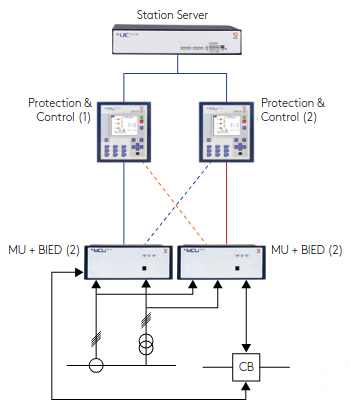
\includegraphics[width=0.77\textwidth, keepaspectratio]{ch3/assets/SLD_Diagram.png}
	\caption{Simple Single Line Diagram (SLD) of an Electrical Substation with SV streams. (Source: Efacec Energia, Máquinas e Equipamentos Eléctricos, S.A.)}
	\label{fig:SLD_Diagram}
\end{figure}

\subsection{Handling Redundancy and Failures}

The proposed solution efficiently manages redundancy by ensuring that the relay always uses the best available data. If one MU fails or its SV stream becomes unreliable, the algorithm automatically switches to the stream with the highest quality, maintaining uninterrupted and accurate protection relay operation. This dynamic handling of redundancy adds an extra layer of resilience to the protection system, preventing erroneous detections and unnecessary interruptions in service.

\section{Conclusion}

In this chapter, we first outlined the configuration and roles of the MUs and protection relays in the substation, explaining how they operate within the context of IEC 61850. We then highlighted the limitations of the current system, particularly the absence of an effective mechanism for selecting the best SV from multiple MUs. Finally, we introduced the architecture of a novel algorithm that dynamically selects the most reliable SV, ensuring higher accuracy and reliability in protection relay operations.






